\documentclass[12pt]{article}

\usepackage{sbc-template}
\usepackage{graphicx,url}
\usepackage[utf8]{inputenc}
\usepackage[brazil]{babel}
\usepackage{listings}
\usepackage[normalem]{ulem}
\useunder{\uline}{\ul}{}
\usepackage{longtable}
\usepackage[justification=centering]{caption}
\usepackage{float}

\lstset{
 numbers=left,
 stepnumber=1,
 firstnumber=1,
 numberstyle=\tiny,
 extendedchars=false,
 breaklines=true,
 frame=single,
 showstringspaces=false,
 xleftmargin=2.5em,
 framexleftmargin=2em,
 basicstyle=\scriptsize,
}

\renewcommand{\lstlistingname}{Código}
\renewcommand{\lstlistlistingname}{Lista de Códigos}

     
\sloppy

\title{Reprodução da Análise Quantitativa de um Experimento}

\author{Diogo C. T. Batista\inst{1}, Elissandra G. Pereira\inst{1}}

\address{Universidade Federal do Paraná (UFPR)\\
 Curitiba -- Paraná -- Brasil
 \email{diogocezar@ufpr.br,egpereira@inf.ufpr.br}
 }

\begin{document}

\maketitle

\begin{resumo}
Este relatório descreve a reprodução da análise quantitativa do experimento apresentado no artigo ``Visual design guidelines for improving learning from dynamic and interactive digital text''. Apresentamos as etapas da análise dos dados no software estatístico e mostramos os resultados obtidos.
\end{resumo}

\section{Identificação do Artigo}

Selecionamos o artigo utilizado anteriormente na atividade de planejamento e execução de um experimento controlado. O artigo comportava as necessidades deste trabalho, apresentando dados brutos de um experimento e seu resultado quantitativo e já estávamos familiarizados com o conteúdo.

O artigo escolhido foi ``Visual design guidelines for improving learning from dynamic and interactive digital text'' \cite{JIN2013248}, que faz uma Análise de Variância Multivariada (MANOVA). Na MANOVA, é possível analisar o efeito de uma ou mais variáveis independentes sobre um conjunto de variáveis dependentes \cite{CHAGAS}

\section{Reconhecimento dos Testes Estatísticos do Experimento}

No artigo, Jin (2013) aplicou testes com estudantes. Os estudantes deveriam ler e tentar entender um texto digital por 20 minutos. Os estudantes completaram então um ``teste de estrutura'' (structure test), um teste de compreensão e um teste de usabilidade.

Para a reprodução e análise exigida no prazo de entrega deste trabalho, decidimos recortar apenas o resultado dos dois primeiros testes. Além disso, os resultados escolhidos foram aqueles relacionados às diretrizes em que tivemos maior interesse e foco em nosso exercício anterior sobre experimentos controlados.

Na Figura \ref{fig:img1} estão dispostos os resultados obtidos por \cite{JIN2013248} em seu artigo. As duas primeiras linhas (Structure e Comprehension) foram escolhidas para nossa reprodução.

\begin{figure}[H]
  \centering
  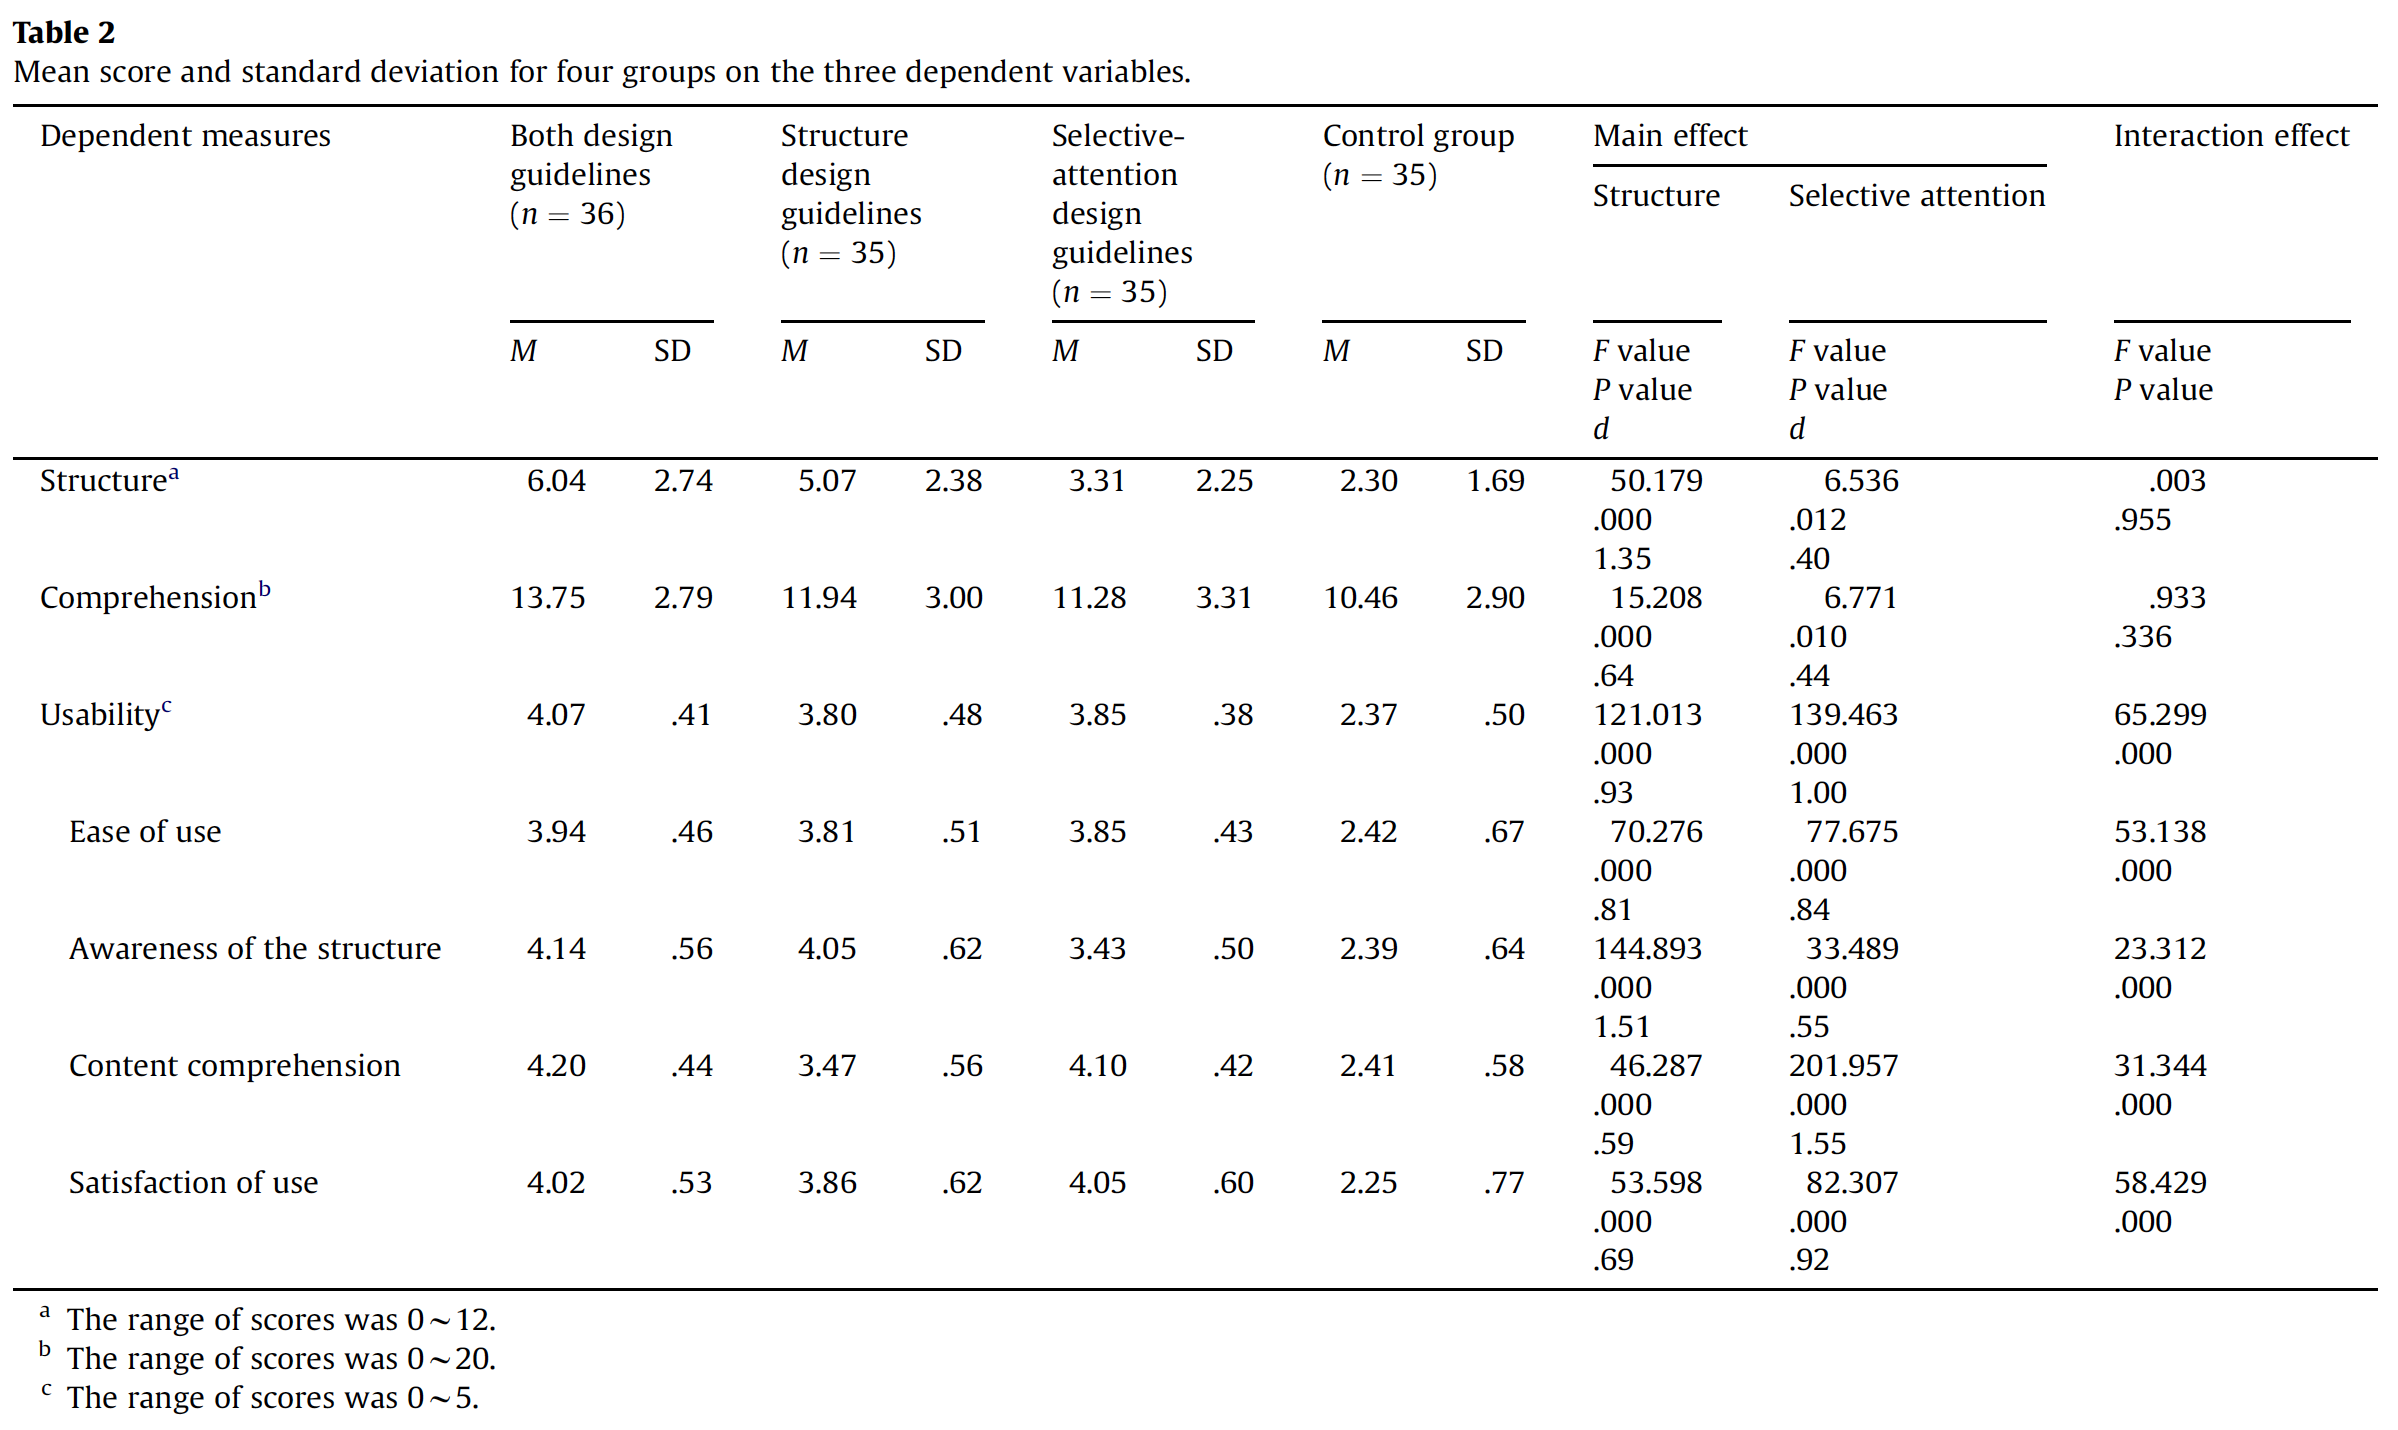
\includegraphics[width=35em]{images/table.png}
  \caption{Resultados utilizados como base}
  \label{fig:img1}
\end{figure}

\section{Reprodução utilizando o software estatístico}

Como o artigo não fornece todas respostas do questionário, gerou-se valores aleatórios com base na média, desvio padrão e número de respostas obtidas, tanto para os testes com \textit{Structure design guidelines}, \textit{Selective-attention design guidelines} e o grupo de controle. Com isso, calculou-se o \textit{valor-p} e o comparamos com os resultado apresentados pelo do autor do artigo. Utilizou-se a estratégia de executar o algoritmo 100 vezes e retirou-se a média de todos os \textit{valor-p} encontrados, para assim podermos termos uma análise melhor para com o resultado descrito no artigo.

\section{Algoritmo Criado}

Para a elaboração do algoritmo utiliou-ze a linguagem \textit{Python}. Em conjunto com as bibliotecas \textit{numpy} e \textit{scipy}

O Código \ref{code:1} mostra a definição de uma função genéria que obtém informações de um grupo qualquer e um grupo controle. São informadas as variáveis:

\begin{itemize}
	\item \texttt{agent\_average}: média do grupo agente;
	\item \texttt{agent\_sigma}: desvio padrão do grupo agente;
	\item \texttt{agent\_num}: quantidade de amostras do grupo agente;
	\item \texttt{control\_average}: média do grupo de controle;
	\item \texttt{control\_sigma}: desvio padrão do grupo de controle;
	\item \texttt{control\_num}: quantidade de amostras do grupo de controle;
	\item \texttt{start}: menor resposta;
	\item \texttt{end}: maior resposta;
	\item \texttt{iterations}: quantas iterações serão realizadas para gerar a média;
\end{itemize}

\begin{lstlisting}[caption={Definição da Função Genérica},language=python,captionpos=b,frame=single,label={code:1}]
import numpy as np
import scipy.stats as stats
 
 def generate(agent_average, agent_sigma, agent_num, control_average, control_sigma, control_num, start, end, iterations):
  values = []
  for x in range(iterations):
   agent_dist = stats.truncnorm((start - agent_average) / agent_sigma, (end - agent_average) / agent_sigma, loc=agent_average, scale=agent_sigma)
   agent_values = agent_dist.rvs(agent_num)
   control_dist = stats.truncnorm((start - control_average) / control_sigma, (end - control_average) / control_sigma, loc=control_average, scale=control_sigma)
   control_values = control_dist.rvs(control_num)
   u_statistic, p_val = stats.mannwhitneyu(agent_values, control_values)
   values.append(p_val)
  return round(np.mean(values), 20)
\end{lstlisting}

Nessa função, obtém-se cada um dos parâmetros, e se gera em um range de \textit{iterations} valores aleatórios que representem a média e o desvio padrão, considerando o grupo de controle nos cálculos.

Para cada uma das iterações, gera-se a distribuição aleatória \texttt{agent\_dist} e \texttt{control\_dist} e obtém-se os seus valores \texttt{agent\_values} e \texttt{control\_values}. Com isso utiliza-se a função \texttt{mannwhitneyu} que abstraí o teste de Mann-Whitney, usado para testar a heterogeneidade de duas amostras ordinais. Os valores retornados são agregados em um vetor, e por fim, retorna-se a média destes valores com um arredondamento.

Na sequência, o Código \ref{code:2} mostra as definições da variáveis de acordo com o trabalho de \cite{JIN2013248}.

\begin{lstlisting}[caption={Definições das Variáveis},captionpos=b,language=python,frame=single,label={code:2}]
 if __name__ == "__main__":
  structure = {
   "control": {
    "average": 2.30,
    "sigma": 1.69,
    "n": 35,
   },
   "structure_design": {
    "average": 5.07,
    "sigma": 2.38,
    "n": 35,
    "start": 0,
    "end": 12
   },
   "selective_attention": {
    "average": 3.31,
    "sigma": 2.25,
    "n": 35,
    "start": 0,
    "end": 12
   },
  }
  comprehension = {
   "control": {
    "average": 10.46,
    "sigma": 2.90,
    "n": 35,
   },
   "structure_design": {
    "average": 11.94,
    "sigma": 3.00,
    "n": 35,
    "start": 0,
    "end": 20
   },
   "selective_attention": {
    "average": 11.28,
    "sigma": 3.31,
    "n": 35,
    "start": 0,
    "end": 20
   },
  }
  result = {
   "structure": {
    "structure_design": generate(
     structure["structure_design"]["average"],
     structure["structure_design"]["sigma"],
     structure["structure_design"]["n"],
     structure["control"]["average"],
     structure["control"]["sigma"],
     structure["control"]["n"],
     structure["structure_design"]["start"],
     structure["structure_design"]["end"],
     100
    ),
    "selective_attention": generate(
     structure["selective_attention"]["average"],
     structure["selective_attention"]["sigma"],
     structure["selective_attention"]["n"],
     structure["control"]["average"],
     structure["control"]["sigma"],
     structure["control"]["n"],
     structure["selective_attention"]["start"],
     structure["selective_attention"]["end"],
     100
    )
   },
   "comprehension": {
    "structure_design": generate(
     comprehension["structure_design"]["average"],
     comprehension["structure_design"]["sigma"],
     comprehension["structure_design"]["n"],
     comprehension["control"]["average"],
     comprehension["control"]["sigma"],
     comprehension["control"]["n"],
     comprehension["structure_design"]["start"],
     comprehension["structure_design"]["end"],
     100
    ),
    "selective_attention": generate(
     comprehension["selective_attention"]["average"],
     comprehension["selective_attention"]["sigma"],
     comprehension["selective_attention"]["n"],
     comprehension["control"]["average"],
     comprehension["control"]["sigma"],
     comprehension["control"]["n"],
     comprehension["selective_attention"]["start"],
     comprehension["selective_attention"]["end"],
     100
    )
   }
  }
  print(result)
\end{lstlisting}

\section{Resultados}

Após a execução do algoritmo, obteve-se resultados disponíveis no Código \ref{code:3}.

\begin{lstlisting}[caption={Saída do script},captionpos=b,frame=single,language=python,label={code:3}]
{
 'structure': {
  'structure_design': 0.0001331037517740879,
  'selective_attention': 0.050186023592034855
 },
 'comprehension': {
  'structure_design': 0.07122011277566724,
  'selective_attention': 0.17129878841709156
 }
}
\end{lstlisting}

A Tabela \ref{tab:resultados} apresenta uma comparação dos resultados obtidos na nossa reprodução da análise e os originais do artigo. Pode-se notar que o resultado obtido para Struture Design (para o tipo Structure) possui equivalência com os apresentados em \cite{JIN2013248}. Os outros três valores possuem maior diferença com os originais devido às limitações do método aplicado de geração de valores aleatórios.

\begin{table}[!htb]
  \centering
	\begin{tabular}{|l|l|l|l|}
		\hline
		\textbf{Experimento} & \textbf{Tipo} & \textbf{pvalue (autor)} & \textbf{pvalue (gerado)} \\ \hline
		Structure Design & Structure & .000 & .000 \\ \hline
		Selective Attention & Structure & .012 & .050 \\ \hline
		Structure Design & Comprehension & .000 & .071 \\ \hline
		Selective Attention & Comprehension & .010 & 0.17 \\ \hline
		\end{tabular}
  \caption{Resultados obtidos na análise}
  \label{tab:resultados}
\end{table}

\section{Conclusão}

A identificação de um artigo que apresente todos os dados brutos necessários para reprodução exigida no trabalho foi uma dificuldade. Como forma de mitigar esta dificuldade, escolhemos o artigo estudado anteriormente para o planejamento e execução de um experimento controlado.

O artigo selecionado apresenta uma rica descrição de diferentes métodos de teste, avaliação e análise em um experimento, além do conteúdo relevante para IHC sobre diretrizes de design em materiais de ensino digital. O estudo feito para este trabalho da disciplina permitiu uma exploração enriquecedora do artigo.

Apesar das limitações causadas pela ausência dos dados brutos, o resultado da reprodução conseguiu replicar de forma satisfatória um dos resultados obtidos pelo trabalho de \cite{JIN2013248}. Percebemos que apesar da reprodução não ter sido ideal, pudemos treinar e estudar de forma adequada o procedimento de análise dos dados.

\bibliographystyle{sbc}
\bibliography{sbc-template}

\end{document}